\documentclass[bigtut]{tutorial}\usepackage[]{graphicx}\usepackage[]{color}
%% maxwidth is the original width if it is less than linewidth
%% otherwise use linewidth (to make sure the graphics do not exceed the margin)
\makeatletter
\def\maxwidth{ %
  \ifdim\Gin@nat@width>\linewidth
    \linewidth
  \else
    \Gin@nat@width
  \fi
}
\makeatother

\definecolor{fgcolor}{rgb}{0.345, 0.345, 0.345}
\newcommand{\hlnum}[1]{\textcolor[rgb]{0.686,0.059,0.569}{#1}}%
\newcommand{\hlstr}[1]{\textcolor[rgb]{0.192,0.494,0.8}{#1}}%
\newcommand{\hlcom}[1]{\textcolor[rgb]{0.678,0.584,0.686}{\textit{#1}}}%
\newcommand{\hlopt}[1]{\textcolor[rgb]{0,0,0}{#1}}%
\newcommand{\hlstd}[1]{\textcolor[rgb]{0.345,0.345,0.345}{#1}}%
\newcommand{\hlkwa}[1]{\textcolor[rgb]{0.161,0.373,0.58}{\textbf{#1}}}%
\newcommand{\hlkwb}[1]{\textcolor[rgb]{0.69,0.353,0.396}{#1}}%
\newcommand{\hlkwc}[1]{\textcolor[rgb]{0.333,0.667,0.333}{#1}}%
\newcommand{\hlkwd}[1]{\textcolor[rgb]{0.737,0.353,0.396}{\textbf{#1}}}%
\let\hlipl\hlkwb

\usepackage{framed}
\makeatletter
\newenvironment{kframe}{%
 \def\at@end@of@kframe{}%
 \ifinner\ifhmode%
  \def\at@end@of@kframe{\end{minipage}}%
  \begin{minipage}{\columnwidth}%
 \fi\fi%
 \def\FrameCommand##1{\hskip\@totalleftmargin \hskip-\fboxsep
 \colorbox{shadecolor}{##1}\hskip-\fboxsep
     % There is no \\@totalrightmargin, so:
     \hskip-\linewidth \hskip-\@totalleftmargin \hskip\columnwidth}%
 \MakeFramed {\advance\hsize-\width
   \@totalleftmargin\z@ \linewidth\hsize
   \@setminipage}}%
 {\par\unskip\endMakeFramed%
 \at@end@of@kframe}
\makeatother

\definecolor{shadecolor}{rgb}{.97, .97, .97}
\definecolor{messagecolor}{rgb}{0, 0, 0}
\definecolor{warningcolor}{rgb}{1, 0, 1}
\definecolor{errorcolor}{rgb}{1, 0, 0}
\newenvironment{knitrout}{}{} % an empty environment to be redefined in TeX

\usepackage{alltt}
\unitcode{MATH1005}
        \unitname{Statistics}
        \semester{Summer/Winter/Semester2}
        \sheetnumber2


\usepackage{graphicx}
\withsolutions
\IfFileExists{upquote.sty}{\usepackage{upquote}}{}
\begin{document}
\lettersfirst

\begin{tutorial}

\begin{center}
\fbox{
\begin{minipage}{7in} 
{\bf Learning in Tutorials}  
\begin{itemize}
\item The role of the tutor is to help you learn more deeply, so the more work you do before the tutorial, the more you will get out of it. 
\item Work at your own pace during the tutorial class and then finish off all the questions at home.   
\item If you finish all the tutorial questions, work on your next Report or the Revision material. 
\end{itemize}
\end{minipage}
}
\end{center}

\vspace{.5cm}
\begin{questions}



\vspace{.5cm}
\question Australian Road Fatalities \\

The following data is road fatalities in Australia from Jan 1989 - May 2016.

\begin{knitrout}
\definecolor{shadecolor}{rgb}{0.969, 0.969, 0.969}\color{fgcolor}\begin{kframe}
\begin{alltt}
\hlstd{Road} \hlkwb{<-} \hlkwd{read.csv}\hlstd{(}\hlstr{"http://www.maths.usyd.edu.au/u/UG/JM/MATH1005/r/StatsData/
                 AllFatalities.csv"}\hlstd{)}
\end{alltt}
\end{kframe}
\end{knitrout}

\vspace{.5cm}
\begin{parts}

\part  What size is the data? How many variables are there? How does this data relate to the example in Topic1 lectures?

\begin{knitrout}
\definecolor{shadecolor}{rgb}{0.969, 0.969, 0.969}\color{fgcolor}\begin{kframe}
\begin{alltt}
\hlkwd{dim}\hlstd{(Road)}
\hlkwd{names}\hlstd{(Road)}
\end{alltt}
\end{kframe}
\end{knitrout}

\vspace{.5cm}
\part  A Data Dictionary gives information about a given data set, such as collection, missing values and variables.
Classify the following variables using the Data Dictionary. \\ 
{\tiny http://www.maths.usyd.edu.au/u/UG/JM/StatsData.html}  \\

\begin{tabular}{|l|l|l|l|l|} \hline
& Numerical & Numerical & Categorical & Categorical \\
Variable & Continuous \hspace{1cm} &  Discrete \hspace{1cm} &  Nominal \hspace{1cm} &  Ordinal \hspace{1cm} \\ \hline
State & & & Y & \\ \hline
Year & & Y & & \\ \hline
Dayweek & &  &  & \\ \hline
CrashType & & &  & \\ \hline
SpeedLimit & & & &  \\ \hline
RoadUser & & & & \\ \hline
Gender & & &  & \\ \hline
Age & & & & \\ \hline
\end{tabular}

\vspace{.5cm}
To check how R has classified the variables, use
\begin{knitrout}
\definecolor{shadecolor}{rgb}{0.969, 0.969, 0.969}\color{fgcolor}\begin{kframe}
\begin{alltt}
\hlkwd{str}\hlstd{(Road)}
\end{alltt}
\end{kframe}
\end{knitrout}

Note: You may have rightly characterised Age as Numerical data, but here R has chosen to classify Age as Categorical Ordinal (factor).

\vspace{.5cm}
\part
Select the Age variable and produce the following graphical summaries:

\begin{knitrout}
\definecolor{shadecolor}{rgb}{0.969, 0.969, 0.969}\color{fgcolor}\begin{kframe}
\begin{alltt}
\hlstd{Age} \hlkwb{<-} \hlstd{Road}\hlopt{$}\hlstd{Age}
\hlkwd{class}\hlstd{(Age)}
\hlkwd{table}\hlstd{(Age)}
\hlkwd{plot}\hlstd{(}\hlkwd{table}\hlstd{(Age))}
\end{alltt}
\end{kframe}
\end{knitrout}

\vspace{.5cm}
\part
Now re-classify the Age variable as numerical data, and then produce the following graphical summaries:

\begin{knitrout}
\definecolor{shadecolor}{rgb}{0.969, 0.969, 0.969}\color{fgcolor}\begin{kframe}
\begin{alltt}
\hlstd{AgeN}\hlkwb{<-} \hlkwd{as.numeric}\hlstd{(}\hlkwd{levels}\hlstd{(Age))[Age]}
\hlkwd{class}\hlstd{(AgeN)}
\hlkwd{hist}\hlstd{(AgeN)}
\hlkwd{boxplot}\hlstd{(AgeN)}
\end{alltt}
\end{kframe}
\end{knitrout}

\vspace{.5cm}
\part
Each command can be customised. Find out the options using \texttt{help()} or \texttt{?}. \\ 


Experiment with customising these commands.

\begin{knitrout}
\definecolor{shadecolor}{rgb}{0.969, 0.969, 0.969}\color{fgcolor}\begin{kframe}
\begin{alltt}
\hlkwd{help}\hlstd{(hist)}
\hlkwd{hist}\hlstd{(AgeN,}\hlkwc{freq}\hlstd{=}\hlnum{FALSE}\hlstd{,}\hlkwc{main}\hlstd{=}\hlstr{"Histogram"}\hlstd{,}\hlkwc{ylab}\hlstd{=}\hlstr{"Probabilities"}\hlstd{,} \hlkwc{col}\hlstd{=}\hlstr{"green"}\hlstd{)}
\hlopt{?}\hlstd{boxplot}
\hlkwd{boxplot}\hlstd{(AgeN,}\hlkwc{horizontal}\hlstd{=}\hlnum{TRUE}\hlstd{,}\hlkwc{col}\hlstd{=}\hlstr{"red"}\hlstd{)}
\end{alltt}
\end{kframe}
\end{knitrout}

\vspace{.5cm}
\part Write a sentence summarising what the histogram and boxplot tell you about the age of road fatalities in Australia (Jan 1989 - May 2016).

\vspace{.5cm}
\part What is the most common and least common days for road fatalities?

\begin{knitrout}
\definecolor{shadecolor}{rgb}{0.969, 0.969, 0.969}\color{fgcolor}\begin{kframe}
\begin{alltt}
\hlstd{Dayweek} \hlkwb{<-} \hlstd{Road}\hlopt{$}\hlstd{Dayweek}
\hlkwd{class}\hlstd{(Dayweek)}
\hlkwd{table}\hlstd{(Dayweek)}
\hlkwd{plot}\hlstd{(}\hlkwd{table}\hlstd{(Dayweek))}
\end{alltt}
\end{kframe}
\end{knitrout}

\vspace{.5cm}
Note to change the labels to shorter names:
\begin{knitrout}
\definecolor{shadecolor}{rgb}{0.969, 0.969, 0.969}\color{fgcolor}\begin{kframe}
\begin{alltt}
\hlkwd{levels}\hlstd{(Dayweek)}
\hlkwd{levels}\hlstd{(Dayweek)} \hlkwb{=} \hlkwd{c}\hlstd{(}\hlstr{"F"}\hlstd{,}\hlstr{"M"}\hlstd{,}\hlstr{"S"}\hlstd{,}\hlstr{"Su"}\hlstd{,}\hlstr{"Th"}\hlstd{,}\hlstr{"T"}\hlstd{,}\hlstr{"W"}\hlstd{)}
\hlkwd{plot}\hlstd{(}\hlkwd{table}\hlstd{(Dayweek))}
\end{alltt}
\end{kframe}
\end{knitrout}

\vspace{.5cm}
\part (Extension:  How can you make more sense of this graph? Reorder the factors alphabetically.)


\begin{knitrout}
\definecolor{shadecolor}{rgb}{0.969, 0.969, 0.969}\color{fgcolor}\begin{kframe}
\begin{alltt}
\hlstd{DayweekOrdered} \hlkwb{<-} \hlkwd{factor}\hlstd{(Dayweek,}\hlkwc{levels}\hlstd{=}\hlkwd{c}\hlstd{(}\hlstr{"M"}\hlstd{,}\hlstr{"T"}\hlstd{,}\hlstr{"W"}\hlstd{,}\hlstr{"Th"}\hlstd{,}\hlstr{"F"}\hlstd{,}\hlstr{"S"}\hlstd{,}\hlstr{"Su"}\hlstd{))}
\hlkwd{plot}\hlstd{(}\hlkwd{table}\hlstd{(DayweekOrdered))}
\end{alltt}
\end{kframe}
\end{knitrout}

\vspace{.5cm}
\part Pick another variable and do your own investigation.
\end{parts}

\vspace{.5cm}
\begin{solution}
This data consists of all Australlian road fatalities from 1989-2016: 46624 fatalities with 18 variables. The data from lectures was just a recent subset of the data: Jan-March 2016.  \\

\begin{tabular}{|l|l|l|l|l|} \hline
& Numerical & Numerical & Categorical & Categorical \\
Variable & Continuous \hspace{1cm} &  Discrete \hspace{1cm} &  Nominal \hspace{1cm} &  Ordinal \hspace{1cm} \\ \hline
State & & & Y & \\ \hline
Year & & Y & & \\ \hline
Dayweek & &  & Y & \\ \hline
CrashType & & & Y & \\ \hline
SpeedLimit & & & & Y \\ \hline
RoadUser & & & Y & \\ \hline
Gender & & & Y & \\ \hline
Age & Y & Y & & Y \\ \hline
\end{tabular}

\vspace{.5cm}
The most common day is Saturday, and then least common day is Monday.
\end{solution}

%\newpage
\question Efficiency of Australian Commercial Refrigerators \\

The following data concerns commercial refrigerators in Australia, in particular the
efficiency (in kWh/24h/m²).

\begin{knitrout}
\definecolor{shadecolor}{rgb}{0.969, 0.969, 0.969}\color{fgcolor}\begin{kframe}
\begin{alltt}
\hlstd{Fridge} \hlkwb{<-} \hlkwd{read.csv}\hlstd{(}\hlstr{"http://www.maths.usyd.edu.au/u/UG/JM/MATH1005/r/StatsData/
                 Refrigerators.csv"}\hlstd{)}
\end{alltt}
\end{kframe}
\end{knitrout}

\vspace{.5cm}
\begin{parts}

\part  What size is the data? How many variables are there? 

\begin{knitrout}
\definecolor{shadecolor}{rgb}{0.969, 0.969, 0.969}\color{fgcolor}\begin{kframe}
\begin{alltt}
\hlkwd{dim}\hlstd{(Fridge)}
\hlkwd{names}\hlstd{(Fridge)}
\end{alltt}
\end{kframe}
\end{knitrout}

\vspace{.5cm}
\part  Classify the following variables using the Data Dictionary. \\ 
{\tiny http://www.maths.usyd.edu.au/u/UG/JM/StatsData.html}  \\

\begin{tabular}{|l|l|l|l|l|} \hline
& Numerical & Numerical & Categorical & Categorical \\
Variable & Continuous \hspace{1cm} &  Discrete \hspace{1cm} &  Nominal \hspace{1cm} &  Ordinal \hspace{1cm} \\ \hline
Brand & & & Y & \\ \hline
Country & &  & & \\ \hline
Sold in & &  &  & \\ \hline
Total energy cons & & & & \\ \hline
Efficiency & & & &  \\ \hline
\end{tabular}

\vspace{.5cm}
\part Comment on the country of manufacture. 

\begin{knitrout}
\definecolor{shadecolor}{rgb}{0.969, 0.969, 0.969}\color{fgcolor}\begin{kframe}
\begin{alltt}
\hlstd{Country} \hlkwb{<-} \hlstd{Fridge}\hlopt{$}\hlstd{Country}
\hlkwd{class}\hlstd{(Country)}
\hlkwd{plot}\hlstd{(Country)}
\hlkwd{table}\hlstd{(Country)}
\end{alltt}
\end{kframe}
\end{knitrout}

\vspace{.5cm}
\part Comment on efficiency.

\begin{knitrout}
\definecolor{shadecolor}{rgb}{0.969, 0.969, 0.969}\color{fgcolor}\begin{kframe}
\begin{alltt}
\hlstd{Efficiency} \hlkwb{<-} \hlstd{Fridge}\hlopt{$}\hlstd{Efficiency..kWh.24h.m..}
\hlkwd{hist}\hlstd{(Efficiency)}
\hlkwd{boxplot}\hlstd{(Efficiency)}
\end{alltt}
\end{kframe}
\end{knitrout}

\vspace{.5cm}
\part Pick another variable and do your own investigation.
\end{parts}

\vspace{.5cm}
\begin{solution}
The data consists of 2480 commerical refrigerators with 23 variables. \\

\begin{tabular}{|l|l|l|l|l|} \hline
& Numerical & Numerical & Categorical & Categorical \\
Variable & Continuous \hspace{1cm} &  Discrete \hspace{1cm} &  Nominal \hspace{1cm} &  Ordinal \hspace{1cm} \\ \hline
Brand & & & Y & \\ \hline
Country & &  & Y & \\ \hline
Sold in & &  & Y  & \\ \hline
Total energy cons & & Y & & \\ \hline
Efficiency & & Y & &  \\ \hline
\end{tabular}

\vspace{.5cm}
The most common countries are: Italy (640) and China (624), followed by New Zealand (314). \\
Efficiency has a right skewed distribution with outliers, indicating some refrigerators have an efficiency far exceeding/worse than the rest.
\end{solution}


\vspace{.5cm}
\question
Investigate demographics in in the USA, using the following Big Data summaries:
http://datausa.io/map/ \\

For example: 

\begin{parts}
\part
What states have the highest and lowest Violent Crime rates?
\part
What states have the highest and lowest Average Salary?
\part
What states have the highest incidence of Diabetes and Obesity?
\end{parts}

\vspace{.5cm}
\begin{solution}
Violent Crime: Tennesee 621.3/100,000 or 0.006213\% (highest); Maine 122.7 (lowest) \\
Average Salary: Columbia  \$72,810.10; Puerto Rico \$25,227 USD. \\
Diabetes: Mississippi 12.5\%; Colorado 6.8\%
Obesity: Mississippi 35.3\%; Colorado 20.1\% \\
\end{solution}



\newpage
\hspace{-1cm} {\bf Extra Questions}

\question Classify Data in Everyday Life \\

For the following scenarios, find appropriate variables. \\

\begin{tabular}{|l|l|l|l|l|} \hline
& Numerical & Numerical & Categorical & Categorical \\
Scenario & Continuous \hspace{1cm} &  Discrete \hspace{1cm} &  Nominal \hspace{1cm} &  Ordinal \hspace{1cm} \\ \hline
Netball Match & & & & \\ \hline
KFC Drive-through & & & & \\ \hline
Hospital & & & & \\ \hline
Masterchef & & & & \\ \hline
\end{tabular}

\vspace{.5cm}
\begin{solution}
{\tiny 
\begin{tabular}{|l|l|l|l|l|} \hline
& Numerical & Numerical & Categorical & Categorical \\
Scenario & Continuous \hspace{1cm} &  Discrete \hspace{1cm} &  Nominal \hspace{1cm} &  Ordinal \hspace{1cm} \\ \hline
Netball Match & Height of players & Number of Goals & Position: Goals/Court & Played which Quarter \\ \hline
KFC Drive-through & Time & Number of Items & Gender of Staff & Rate service \\ \hline
Hospital & Age of building & Number of staff & State & Cleanliness standard \\ \hline
Masterchef & Quantity of cream & Number of contestants & Type of dish & What Star Chef  \\ \hline
\end{tabular}
}
\end{solution}



\question True heat of Platinum \\

In an attempt to measure the `true' heat of sublimation of platinum (in kcal/mole),
Hampson and Walker (1961) recorded the following data:

\begin{center}
\begin{tabular}{llllllll}
136.2&136.6&135.8&135.4&134.7&135.0&134.1&143.3 \\
147.8&148.8&134.8&135.2&134.9&146.5&141.2&135.4 \\
134.8&135.8&135.0&133.7&134.2&134.9& 134.8 & 134.5 \\
134.3 & 135.2 &&&&&&
\end{tabular}
\end{center}
{\tiny Source: http://nvlpubs.nist.gov/nistpubs/jres/65A/jresv65An4p289\_A1b.pdf} 

\vspace{.5cm}
\begin{parts}
\part Who would be interested in ths data and why?
\part
Import the data into R.
\begin{knitrout}
\definecolor{shadecolor}{rgb}{0.969, 0.969, 0.969}\color{fgcolor}\begin{kframe}
\begin{alltt}
\hlstd{Plat}\hlkwb{=}\hlkwd{scan}\hlstd{(}\hlkwc{file}\hlstd{=}\hlkwd{url}\hlstd{(}\hlstr{"http://www.maths.usyd.edu.au/u/UG/JM/MATH1005/r/StatsData/
                Platinum.txt"}\hlstd{))}
\end{alltt}
\end{kframe}
\end{knitrout}

\part Produce graphical summaries and comment on your results.
\begin{knitrout}
\definecolor{shadecolor}{rgb}{0.969, 0.969, 0.969}\color{fgcolor}\begin{kframe}
\begin{alltt}
\hlkwd{stem}\hlstd{(Plat)}
\hlkwd{stem}\hlstd{(Plat,}\hlkwc{scale}\hlstd{=}\hlnum{2}\hlstd{)}
\hlkwd{hist}\hlstd{(Plat,}\hlkwc{breaks}\hlstd{=}\hlkwd{c}\hlstd{(}\hlnum{133}\hlopt{:}\hlnum{137}\hlstd{,}\hlnum{140}\hlstd{,}\hlnum{143}\hlstd{,}\hlnum{146}\hlstd{,}\hlnum{149}\hlstd{),}\hlkwc{right}\hlstd{=F)}
\hlkwd{hist}\hlstd{(Plat,}\hlkwc{breaks}\hlstd{=}\hlkwd{c}\hlstd{(}\hlnum{133}\hlopt{:}\hlnum{137}\hlstd{,}\hlnum{140}\hlstd{,}\hlnum{143}\hlstd{,}\hlnum{146}\hlstd{,}\hlnum{149}\hlstd{),}\hlkwc{right}\hlstd{=F)}\hlopt{$}\hlstd{counts}
\end{alltt}
\end{kframe}
\end{knitrout}

Note:  \\
(1) R chooses what it considers to be an appropriate spread of the stem and leaf plot. So we use the parameter \texttt{scale =} to change the default layout. In this particular example, using \textsf{scale = 2} produces a single stem plot. \\

(2) \texttt{\$counts} adds the counts per interval.

\part Now complete the graphical summaries by hand. Complete the following unsorted `single' stem and leaf plot, where the break is at the decimal point.  The first 5 entries have been done already.   \\

\begin{center}
\begin{tabular}{l | l} 
133 &  \\ 
134 & 7 \\
135 & 8 4 \dots \\
136 & 2  6 \dots \\
\vdots &  \\
\vdots &  \\
\vdots &  \\
148 &  \\
\end{tabular}
\end{center}

Note: The single stem version has 10 digits/leaves on each row/stem.


\part
Complete the following frequency table, and draw a histogram. \\

\begin{center}
\begin{tabular}{|l |l |l |l |} \hline
Interval & Frequency & Relative Frequency (3dp) & Height  (3dp)  \\ \hline
[133,134) & 1 & 0.038 & 0.038  \\ \hline
[134,135) & 10  &   &   \\ \hline
[135,136) & & &  \\ \hline
[136,137) & & &  \\ \hline
[137,140) & & &  \\ \hline
[140,143) & & &  \\ \hline
[143,146) & & &  \\ \hline
[146,149) & 3 & 0.115 & 0.038   \\ \hline
Total & & &  \\ \hline
\end{tabular}
\end{center}

where: \\
Relative Frequency = Frequency/Total \\
Height = Relative Frequency/Interval Width
\end{parts}


\vspace{.5cm}
\begin{solution}
Data could be of interest to anyone using Platinum commercially. The shape is right skewed (long right tail), indicating some very high values of  'true' heat relative to the rest of data, which could be investigated further.
\end{solution}




\begin{solution}

Check your hand working against the following R output.

\vspace{.5cm}
\begin{tabular}{|c |c |c |c |} \hline
Interval & Frequency & Relative Frequency \% & Height \\ \hline
[133,134) & 1 & 1/26 = 3.8 & 3.8/1=3/8  \\ \hline
[134,135) & 10 & 10/26 = 38.5 &  38.5/1=38.5  \\ \hline
[135,136) & 8 & 8/26 =  30.1 & 30.1/1=30.1  \\ \hline
[136,137) & 2 & 2/26 = 7.7 &  7.7/1=7.7  \\ \hline
[137,140) & 0 & 0 & 0/3=0 \\ \hline
[140,143) & 1 & 1/26 = 3.8 & 3.8/3 $\approx$ 1.3  \\ \hline
[143,146) & 1 & 1/26 = 3.8  & 3/8/3 $\approx$ 1.3 \\ \hline
[146,149) & 3  & 3/26 =  11.5 & 11.5/3 $\approx$ 3.8  \\ \hline
Total & 26 &  100 (rounding) & \\ \hline
\end{tabular}
\end{solution}


\question Mining Core Samples  (From the 1998 examination)  \\

A mining company finds a body of ore and obtains 24 core samples by drilling at equally spaced intervals along the body. The samples are analysed for percentage content of a valuable mineral giving the following results:


  \begin{center}
  \begin{tabular}{llllllll}
 17&18&26&18&31&31&19&17\\
 22&13&19&17&16&14&13&10\\
 16&14&13&23&16&20&18&30
 \end{tabular}
   \end{center}
                       
Prepare both single and double stem-and-leaf plots. Which one is preferable and why? \\

Note: The double stem version has 5 digits/leaves on each row/stem. 




\begin{solution}
Check your working against the following R output.
\begin{knitrout}
\definecolor{shadecolor}{rgb}{0.969, 0.969, 0.969}\color{fgcolor}\begin{kframe}
\begin{alltt}
\hlstd{x}\hlkwb{=}\hlkwd{c}\hlstd{(}\hlnum{17}\hlstd{,}\hlnum{18}\hlstd{,}\hlnum{26}\hlstd{,}\hlnum{18}\hlstd{,}\hlnum{31}\hlstd{,}\hlnum{31}\hlstd{,}\hlnum{19}\hlstd{,}\hlnum{17}\hlstd{,}\hlnum{22}\hlstd{,}\hlnum{13}\hlstd{,}\hlnum{19}\hlstd{,}\hlnum{17}\hlstd{,}\hlnum{16}\hlstd{,}\hlnum{14}\hlstd{,}\hlnum{13}\hlstd{,}\hlnum{10}\hlstd{,}\hlnum{16}\hlstd{,}\hlnum{14}\hlstd{,}\hlnum{13}\hlstd{,}\hlnum{23}\hlstd{,}\hlnum{16}\hlstd{,}\hlnum{20}\hlstd{,}\hlnum{18}\hlstd{,}\hlnum{30}\hlstd{)}
\hlkwd{stem}\hlstd{(x)}
\end{alltt}
\begin{verbatim}
## 
##   The decimal point is 1 digit(s) to the right of the |
## 
##   1 | 033344
##   1 | 66677788899
##   2 | 023
##   2 | 6
##   3 | 011
\end{verbatim}
\begin{alltt}
\hlkwd{stem}\hlstd{(x,}\hlkwc{scale}\hlstd{=}\hlnum{0.5}\hlstd{)}
\end{alltt}
\begin{verbatim}
## 
##   The decimal point is 1 digit(s) to the right of the |
## 
##   1 | 03334466677788899
##   2 | 0236
##   3 | 011
\end{verbatim}
\end{kframe}
\end{knitrout}
  
Note: Here by default R chooses a double stem and leaf plot. Hence,we use \texttt{scale=0.5} to get a single stem and leaf plot. \\

Comment: The double stem plot is preferable, because it's easier to see the shape (some right skewing). The single stem plot is a bit overcondensed.
\end{solution}


\question Icecreams in Canada \\

The following table gives the number of ice creams sold in a coffee shop
on each day in January 2002 in a Canadian city:
\begin{center}
 \begin{tabular}{llllllll}
   2&0&0&1&1&0&2&1\\
 3&3&6&7&0&4&1&0\\
1&1&3&2&1&0&8&0\\
  0&4&5&1&0&2&3&
 \end{tabular}
\end{center}

Prepare a suitable frequency distribution table for this data. Draw an ordinate
diagram and comment.


\begin{solution}

Check your working against the following R output.
\begin{knitrout}
\definecolor{shadecolor}{rgb}{0.969, 0.969, 0.969}\color{fgcolor}\begin{kframe}
\begin{alltt}
\hlstd{x}\hlkwb{=}\hlkwd{c}\hlstd{(}\hlnum{2}\hlstd{,}\hlnum{0}\hlstd{,}\hlnum{0}\hlstd{,}\hlnum{1}\hlstd{,}\hlnum{1}\hlstd{,}\hlnum{0}\hlstd{,}\hlnum{2}\hlstd{,}\hlnum{13}\hlstd{,}\hlnum{3}\hlstd{,}\hlnum{6}\hlstd{,}\hlnum{7}\hlstd{,}\hlnum{0}\hlstd{,}\hlnum{4}\hlstd{,}\hlnum{1}\hlstd{,}\hlnum{0}\hlstd{,}\hlnum{1}\hlstd{,}\hlnum{1}\hlstd{,}\hlnum{3}\hlstd{,}\hlnum{2}\hlstd{,}\hlnum{1}\hlstd{,}\hlnum{0}\hlstd{,}\hlnum{8}\hlstd{,}\hlnum{0}\hlstd{,}\hlnum{0}\hlstd{,}\hlnum{4}\hlstd{,}\hlnum{5}\hlstd{,}\hlnum{1}\hlstd{,}\hlnum{0}\hlstd{,}\hlnum{2}\hlstd{,}\hlnum{3}\hlstd{)}
\hlkwd{table}\hlstd{(x)}
\end{alltt}
\begin{verbatim}
## x
##  0  1  2  3  4  5  6  7  8 13 
##  9  7  4  3  2  1  1  1  1  1
\end{verbatim}
\begin{alltt}
\hlkwd{plot}\hlstd{(}\hlkwd{table}\hlstd{(x),}\hlkwc{xlab}\hlstd{=}\hlstr{"Icecreams"}\hlstd{,} \hlkwc{ylab}\hlstd{=}\hlstr{"Frequency"}\hlstd{,}\hlkwc{main}\hlstd{=}\hlstr{"Ordinate Diagram"}\hlstd{)}
\end{alltt}
\end{kframe}
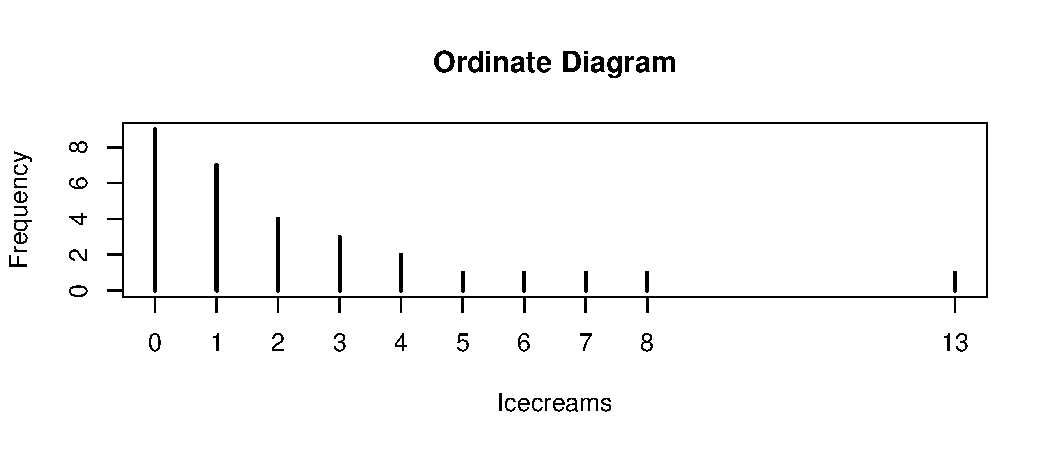
\includegraphics[width=\maxwidth]{figure/unnamed-chunk-17-1} 

\end{knitrout}

Comment: The data is right skewed, indicating there are many days when very few icecreams are sold, as might be expected given climate. 

\end{solution}

\end{questions}
\end{tutorial}
\end{document}

